\chapter{Results} 

\label{Chapter7} 

\lhead{Chapter 7. \emph{Results}}

\section{Performance}
\label{sec:performanceanalysis}
Performance has been the main concern in the development of the system. As already seen in previous chapters, many efforts have been made in order to achieve a good responsiveness to user input in the real time application. We made the clear choice of preferring low times in the offline computation of descriptors (reported in Table~\ref{table:benchmarkoffline}) for this has helped us in achieving good response times in the real time application. Response times were controlled in order to provide the fastest response while preserving the quality of the retrieval: when the user moves sliders, the playlist queue gets empty (which will result in temporary shorter computational times, due to the use of the least precise but fastest music similarity computation algorithm in order to get some new element into the playlist as soon as possible); contrastringly, when the user chooses long segments or does not interact with the sliders, the computational time may increase (for the system realizes that it has more time available for computing music similarity and then uses the most accurate algorithm\footnote{We recall that the only difference between the two algorithms lies in the choice of the similarity function, as shown at the point 8 of Section~\ref{subsec:rtalgorithm}}). \\
In other words, we have built an \textit{adaptive} system, defined in \cite{stober11} as a system that:
\begin{itemize}
\item Behaves different in different contexts given the same input, and
\item Performs this adaptation in order to optimize the system's behaviour in the given context according to some predefined measure.
\end{itemize}
In order to analyze its performance, we decided to collect data about computational times of the real time application for the choice of 1000 consecutive excerpts, with occasional interaction of the user. This is a reasonable analysis case, for it may be very similar to the real use of the system and also provides a good perspective on the computational times while using the most demanding algorithm of the system for computing music similarity. The hardware used in this analysis is the one reported in Table~\ref{table:hardwareoffline}. Values of the global times required for choosing these 1000 consecutive excerpts are shown in Figure~\ref{fig:step7}. 

\begin{figure}[h]
\begin{center}
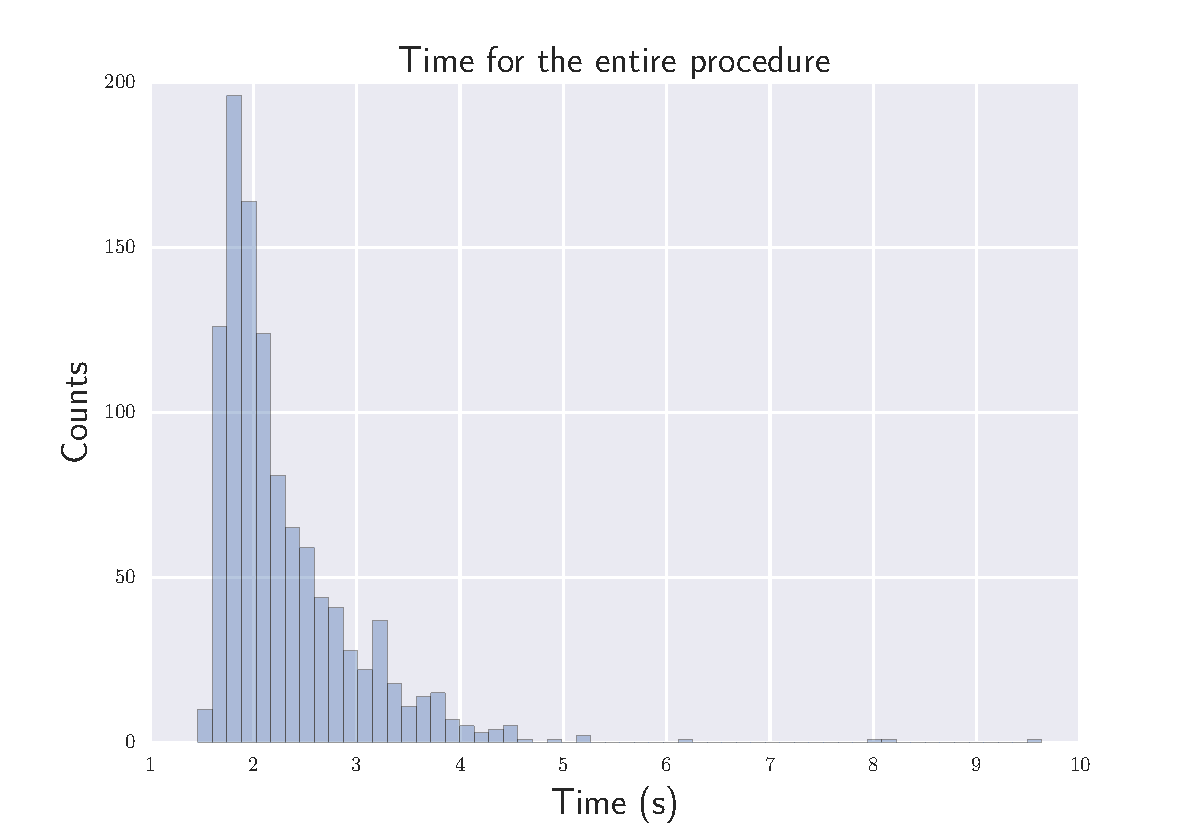
\includegraphics[scale=0.7]{Figures/bench_procedure.pdf}
    % \rule{10em}{0.5pt}
  \caption[Global times for selecting next segment]{Global times for selecting next segment.}
  \label{fig:step7}
\end{center}
\end{figure}

It can be seen that most of the times, the algorithm for choosing the next excerpt requires between 1.5 seconds and 3 seconds. The presence of some outliers above 5 seconds is due to particular conditions of the environment or of the operative system (such as some other process starting running in the background) and should not be considered meaningful for judging the performance of the algorithm itself. \\
We consider particularly valuable that the system is capable of adapting its responsiveness to the environment, while still getting good response times also with most intensive computations. As already stated, during this  experiment user interactions were occasional, leading the system to use the most intensive (but more precise regarding to retrieval) variant of the algorithm 732 out of 1000 times.\\ 
We will now discuss the computational times required for individual steps of the procedure presented in Section~\ref{subsec:rtalgorithm}. The first step consists of selecting, among all the excerpts of the Phonos catalogue of music, the ones that fulfill the current sliders' values. For this step has to compare several values of all the 159239 excerpts, it is the most demanding task of the algorithm, requiring around 1.6 seconds.

\begin{figure}[htbp]
\begin{center}
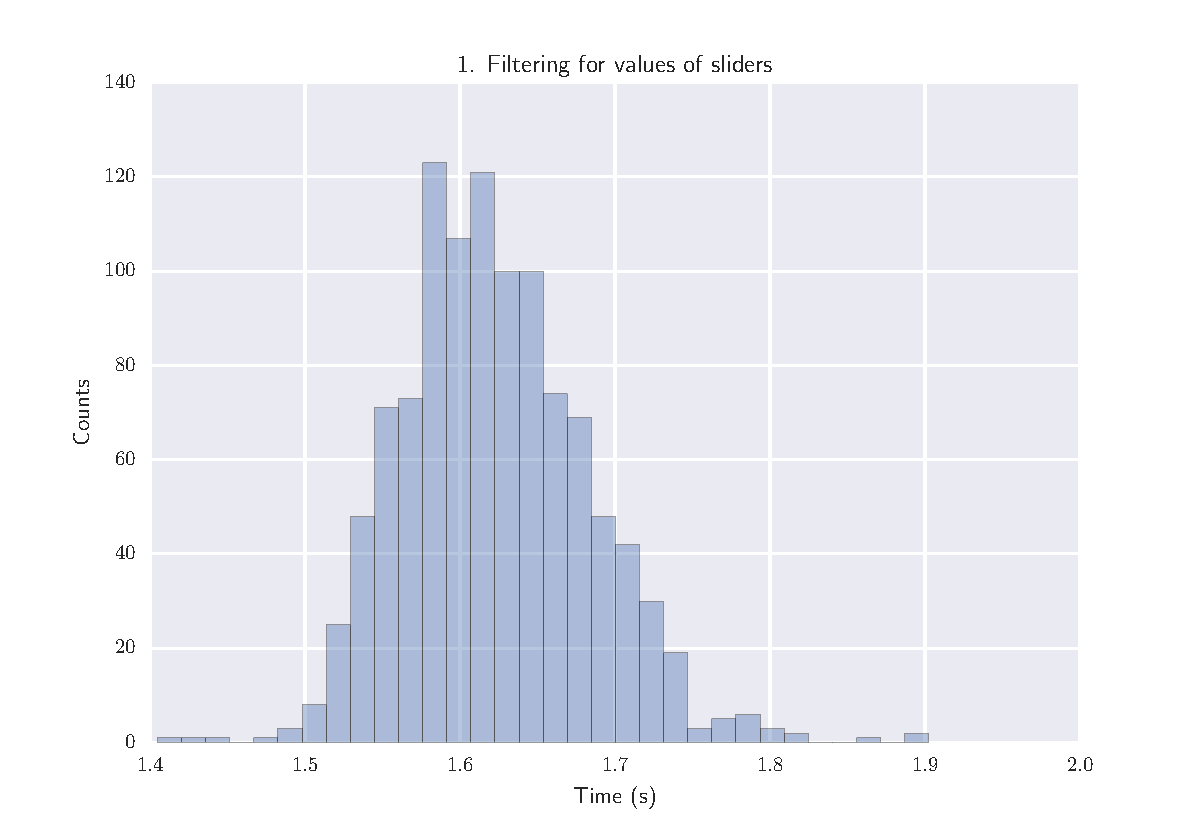
\includegraphics[scale=0.7]{Figures/bench_sliders.pdf}
    % \rule{10em}{0.5pt}
  \caption[Time for filtering music in regards to sliders' positions]{Time for performing the first step of the procedure: filtering of excerpts based on the current positions of sliders.}
  \label{fig:step1}
\end{center}
\end{figure}

The next two steps consist of further filtering of candidate excerpts: at first a Monte Carlo sampling is performed to further reduce the size of the problem, and then we filter out candidate segments that would be generate a quite dissonant result if mixed with the previous excerpt of the playlist. It can be seen the both these operations are much faster than the first one, although the Monte Carlo sampling still requires a tiny considerable time (around 0.02 seconds). \\ \vspace{5.5cm}

\begin{figure}[htbp]
\begin{center}
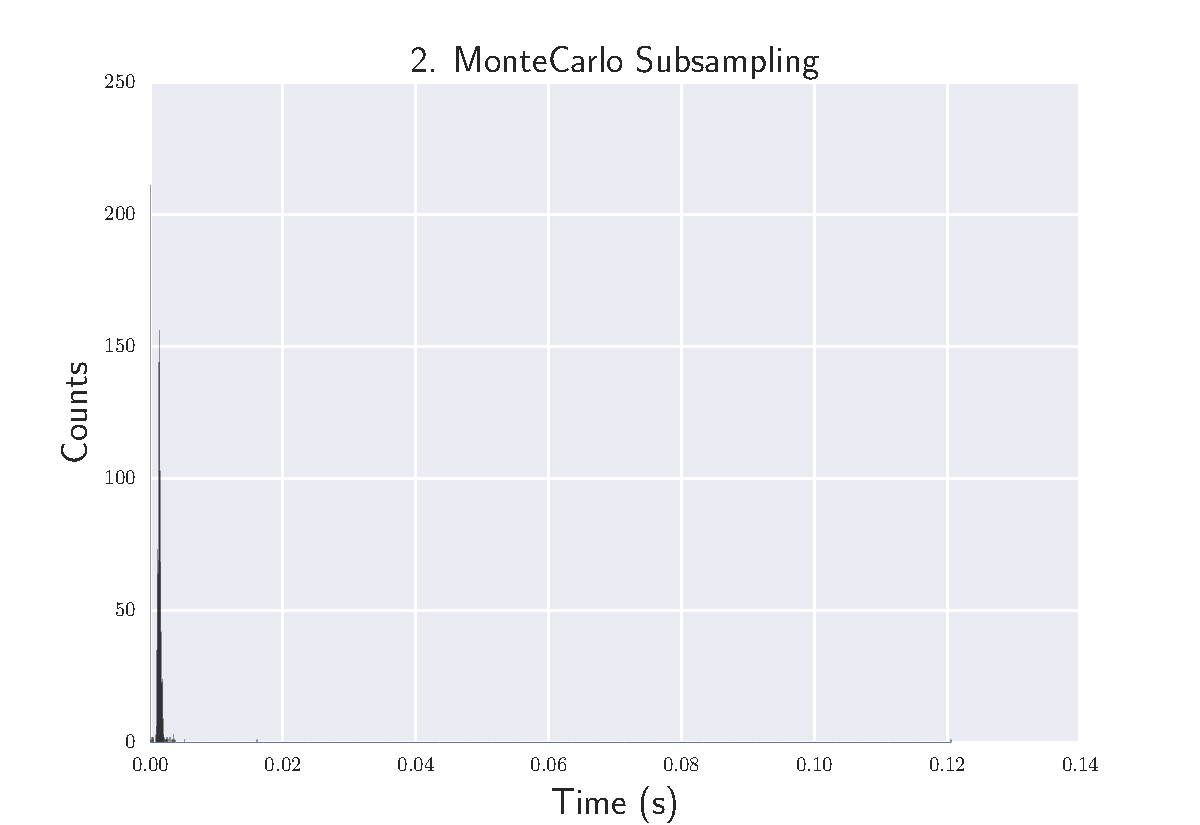
\includegraphics[scale=0.7]{Figures/bench_subsampling.pdf}
    % \rule{10em}{0.5pt}
  \caption[Time for performing Monte Carlo sampling]{Time for performing Monte Carlo sampling.}
  \label{fig:step2}
\vspace{2cm}
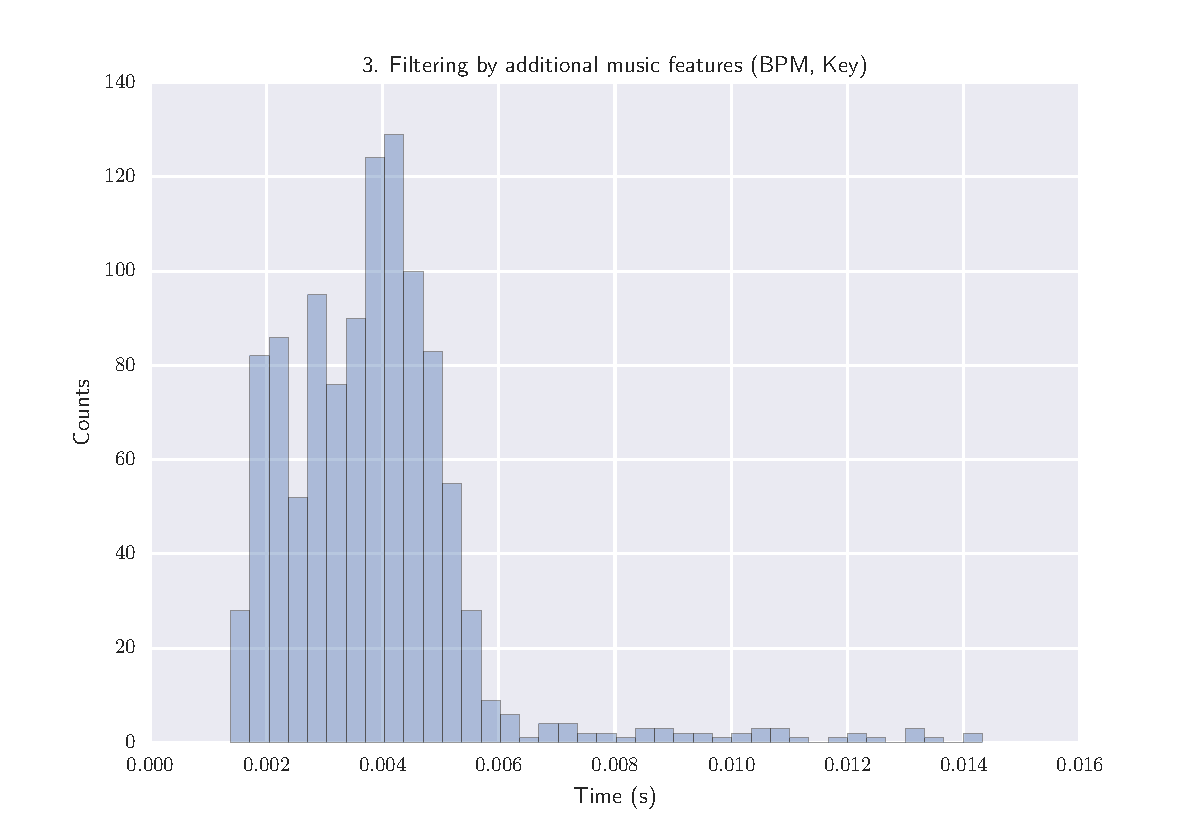
\includegraphics[scale=0.7]{Figures/bench_bpm_filters.pdf}
    % \rule{10em}{0.5pt}
  \caption[Time for filtering music according to musicality with current excerpt]{Time for filtering music according to musicality with current excerpt (in regards of BPM and key).}
  \label{fig:step3}
\end{center}
\end{figure}

At this point, a context-aware distance function is applied to select the next excerpt of the playlist among all the remaining candidates. According to the context, a simple Euclidean distance or a more complex Kullback-Leibler divergence may be computed, and from the following graphs we can see the difference in the computational times of the two:

\begin{figure}[htbp]
\begin{center}
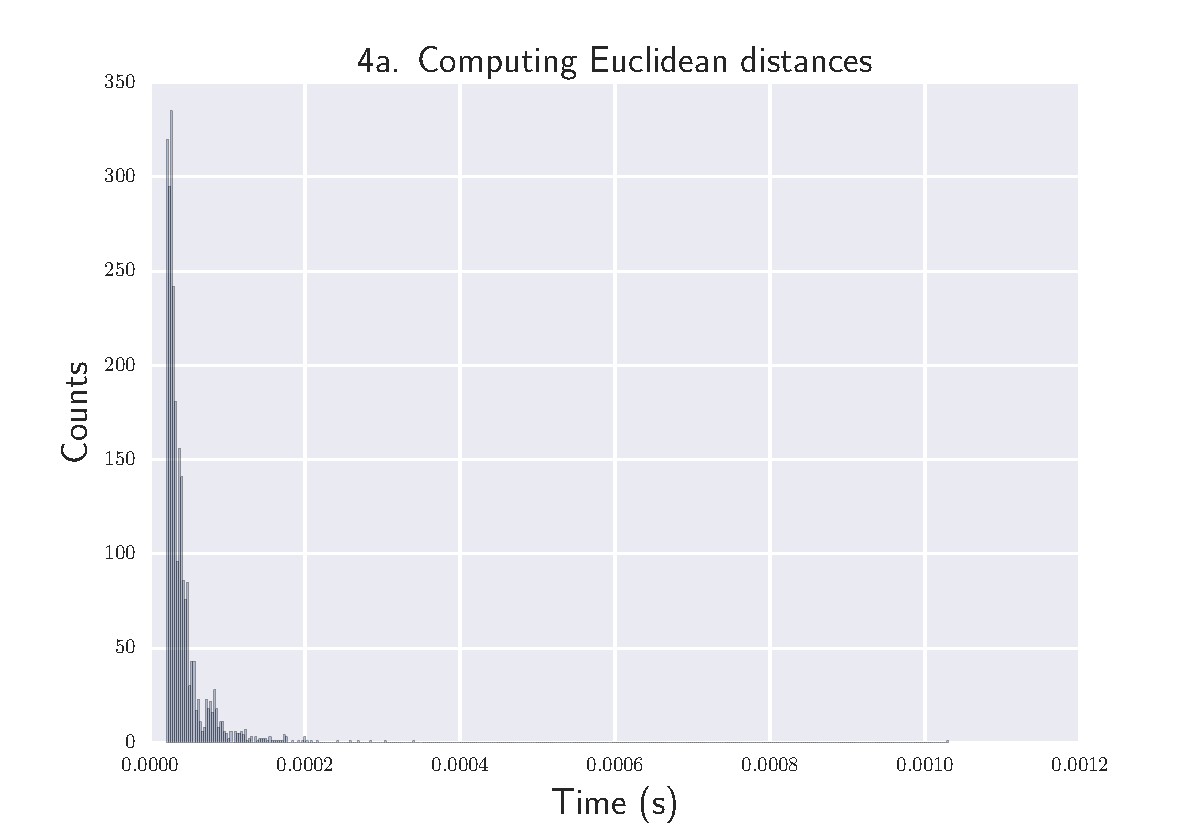
\includegraphics[scale=0.6]{Figures/bench_euclidean.pdf}
    % \rule{10em}{0.5pt}
  \caption[Time for computing euclidean distance]{Time for computing euclidean distance between two 20D points.}
  \label{fig:step4}
\vspace{1cm}
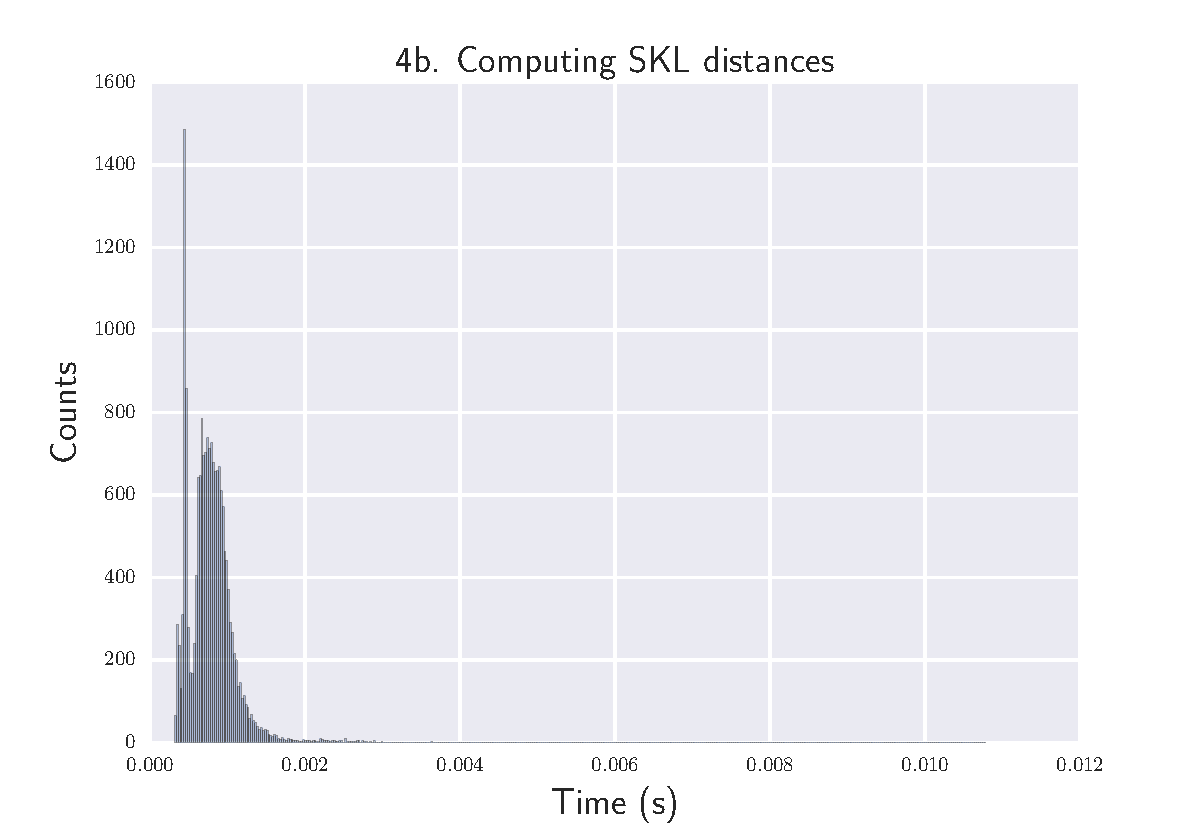
\includegraphics[scale=0.6]{Figures/bench_skl.pdf}
    % \rule{10em}{0.5pt}
  \caption[Time for computing symmetric Kullback-Leibler distance]{Time for computing symmetric Kullback-Leibler divergence between the single Gaussian distributions of the MFCCs values of two excerpts.}
  \label{fig:step5}
\end{center}
\end{figure}

The global times for computing the distance between all the remaining candidates and the last excerpt of the playlist are shown in Figure~\ref{fig:step6}. It is important to remark that the values of the single Gaussian distributions are stored on JSON files; therefore the computation of KL divergence requires the access to these files. The time required for accessing and parsing these files is shown in Figure~\ref{fig:step8}.
\begin{figure}[htbp]
\begin{center}
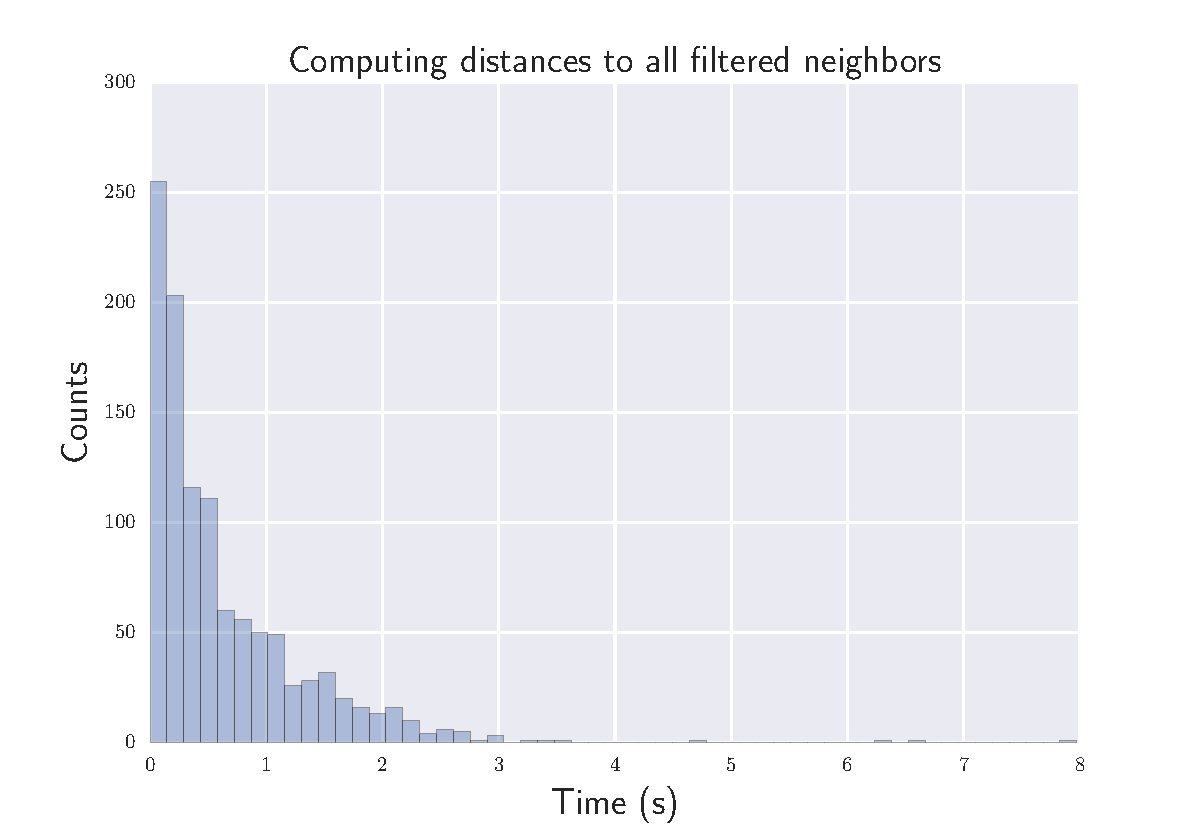
\includegraphics[scale=0.6]{Figures/bench_get_suitsegm.pdf}
    % \rule{10em}{0.5pt}
  \caption[Time for computing distances from all filtered segments]{Time for computing distances from all filtered segments.}
  \label{fig:step6}
\vspace{1cm}
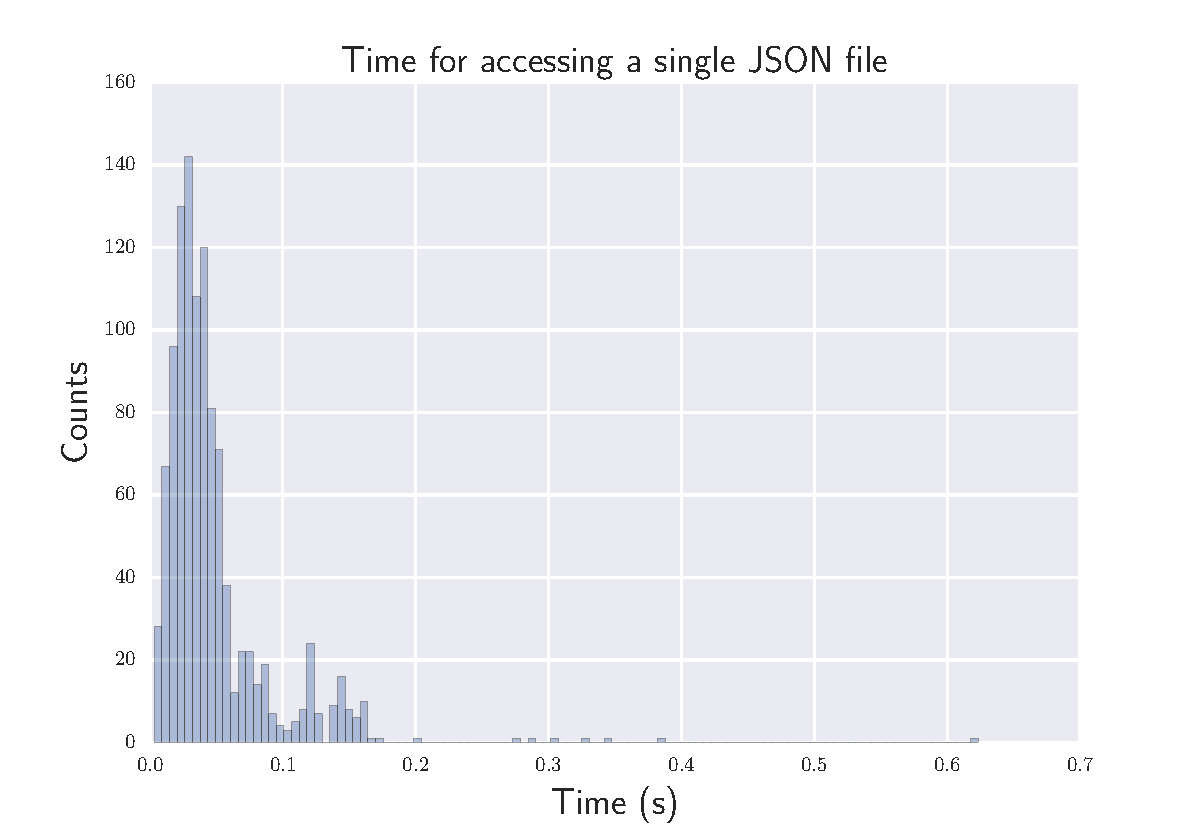
\includegraphics[scale=0.6]{Figures/bench_json_single.pdf}
    % \rule{10em}{0.5pt}
  \caption[Time for accessing and parsing a JSON file]{Time for accessing and parsing a JSON file.}
  \label{fig:step8}
\end{center}
\end{figure}

Looking at these graphs, several details emerge:
\begin{itemize}
\item Without any doubt, the most demanding task is the filtering of candidates on the base of sliders value. This is due to the fact that this is step acting on the highest number of excerpts. This filtering is based on values that are stored on RAM and therefore is not sensibly slowed down by the time for accessing these values. 
\item Random sampling, having possibly to act on a very large collection of excerpt, is one of the longest tasks.
\item Once all the filtering steps are done, computing all the similarity distances generally requires around one second. 
\item Computing symmetric Kullback-Leibler distance is around 10 times slower then computing Euclidean distance.
\item Time for accessing and parsing JSON file is not negligible and is actually 100 times longer than computing the symmetric Kullback-Leibler distance.
\end{itemize}

\section{User evaluation}
\label{sec:eval_results}
As explained in Section~\ref{sec:evaluation_idea}, we have decided to perform the evaluation of the system with learn-play-discuss sessions, followed by the compilation of a survey.
Specifically, the evaluation sessions are organized as follows:
\begin{itemize}
\item The subject of the experiment is introduced to the purpose of the application, without explaining any details about the interaction or the functioning;
\item The subject is given 5 minutes to freely interact with the application (playing with the Phonos collection of music), asking for clarification about the use if necessary;
\item The subject is finally given the chance to ask about more the functioning of the system;
\item The subject answers the survey (presented in Appendix~\ref{AppendixD}) with specific questions about ease of usage, enjoyment of musical output, familiarity with the music and with this kind of software, and any problems. 
\end{itemize}

19 subjects took part to this evaluation, recruited from members of the Music Technology Group of Universitat Pompeu Fabra, Barcelona. The subjects were all male, aged between 24 and 34. \\ \vspace{0.5cm}
The application was generally evaluated very easy to use, with 13 subjects considering it extremely easy: \\
\begin{figure}[h]
\begin{center}
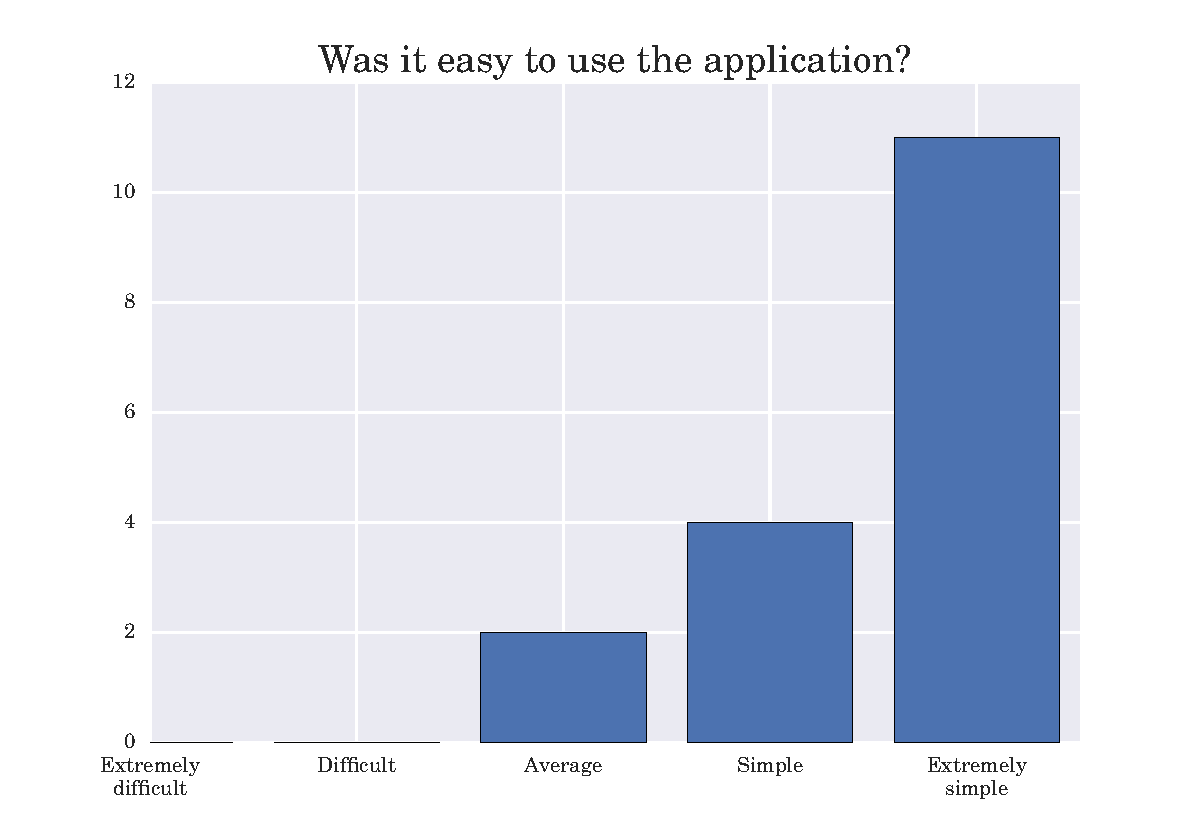
\includegraphics[scale=0.7]{Figures/easytouse.pdf}
  \caption[Evaluation results: ease of use]{Evaluation results: ease of use.}
\end{center}
\end{figure}
\\
despite many of them not having used any similar software before: \\
\begin{figure}[h]
\begin{center}
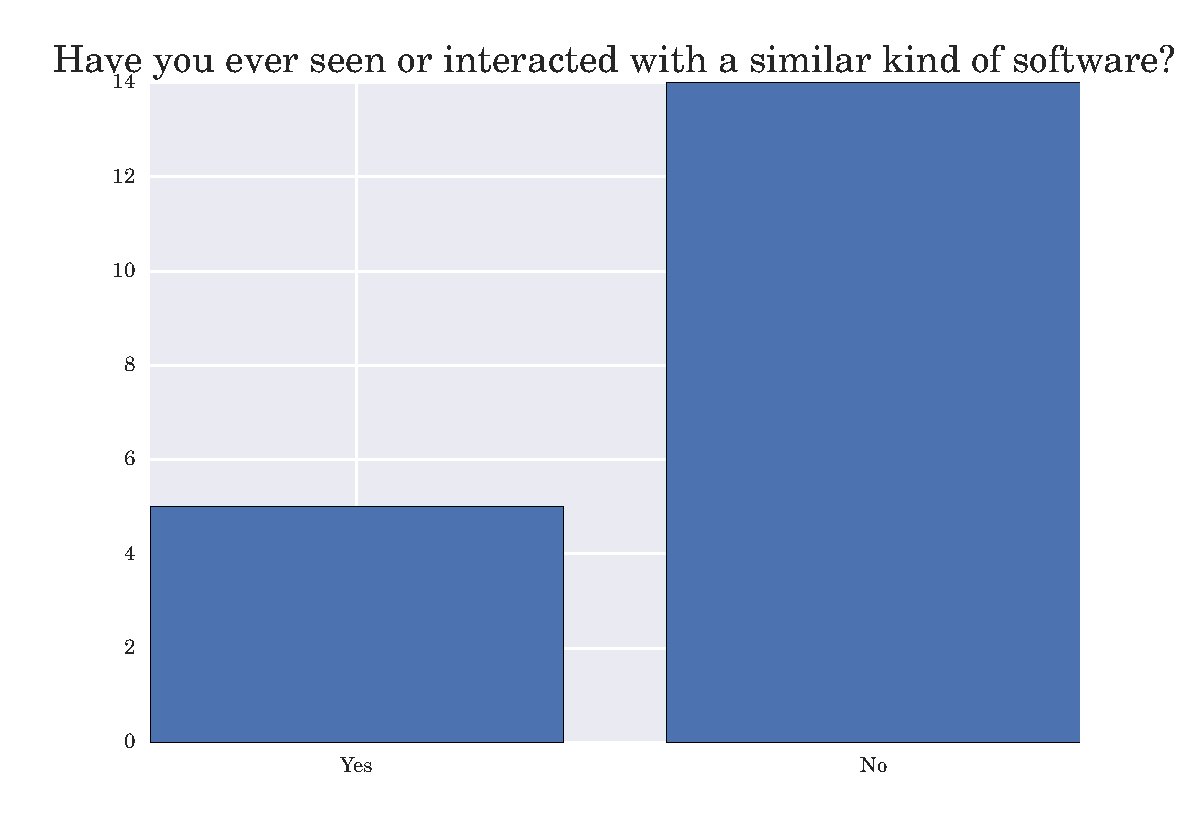
\includegraphics[scale=0.52]{Figures/similarsoftware.pdf}
  \caption[Evaluation results: familiarity with software]{Evaluation results: familiarity with software.}
\end{center}
\end{figure}

The meaning of the sliders was generally understood, and the output was evaluated mainly enjoyable and ``flowing'', despite general lack of familiarity with the music genre:\\
\begin{figure}[h]
\begin{center}
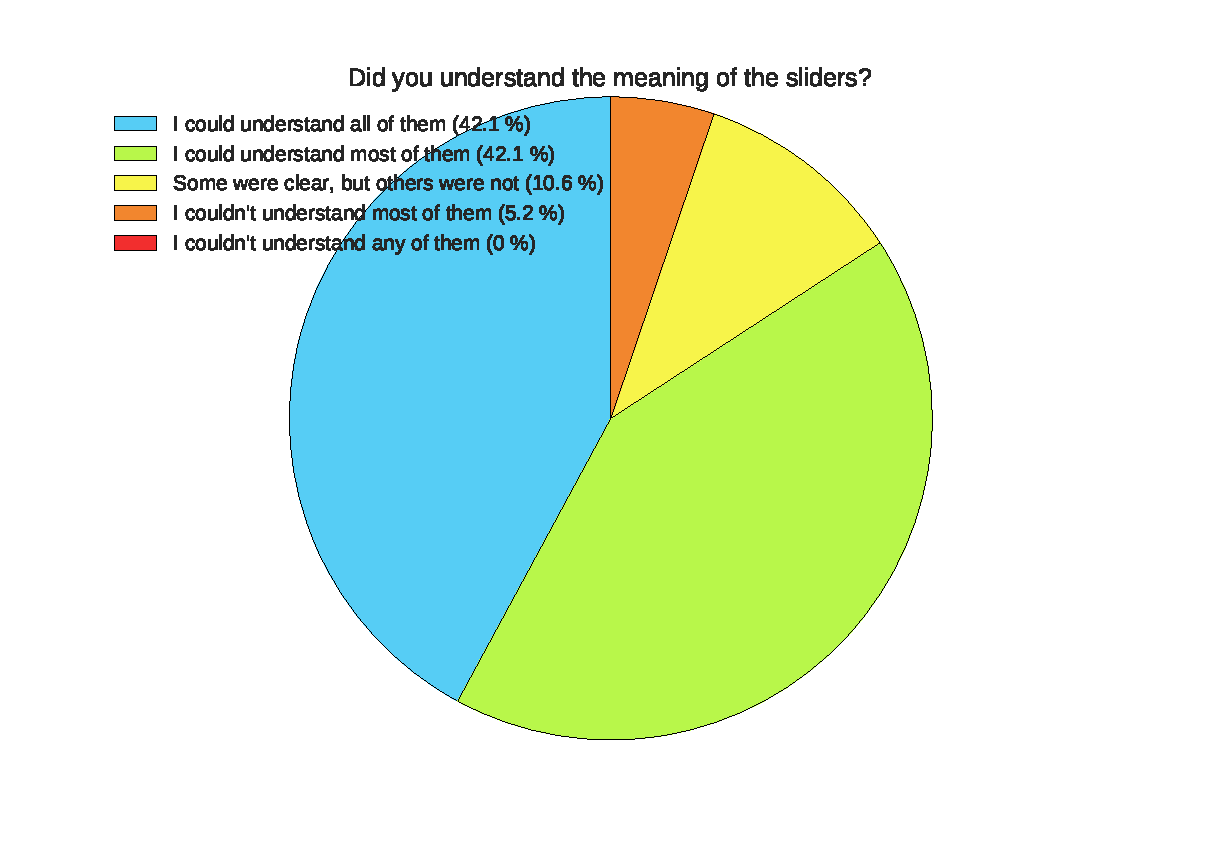
\includegraphics[scale=0.67]{Figures/slidersmeaning.pdf}
  \caption[Evaluation results: understanding of sliders' meaning]{Evaluation results: understanding of sliders' meaning.}
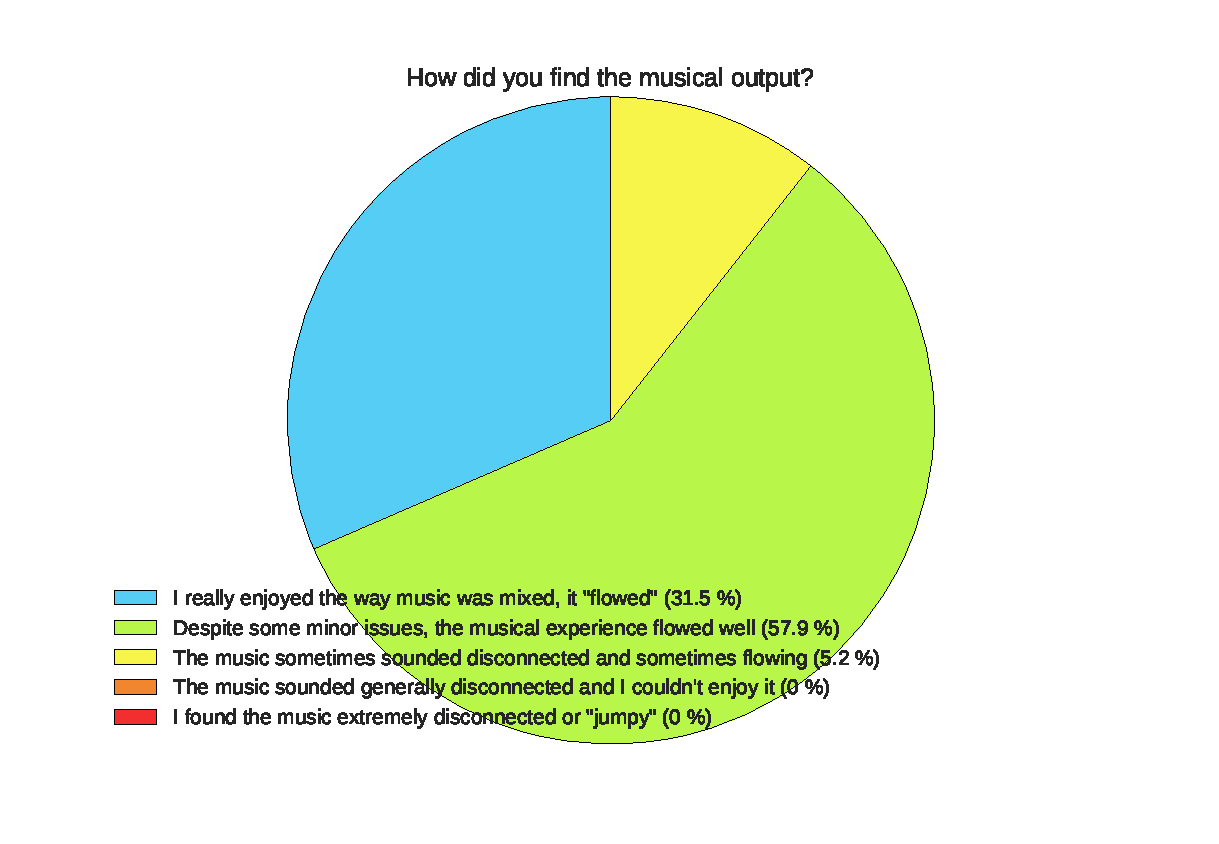
\includegraphics[scale=0.67]{Figures/flow.pdf}
  \caption[Evaluation results: enjoyability of musical output]{Evaluation results: enjoyability of musical output.}
\end{center}
\end{figure}

\begin{figure}[h]
\begin{center}
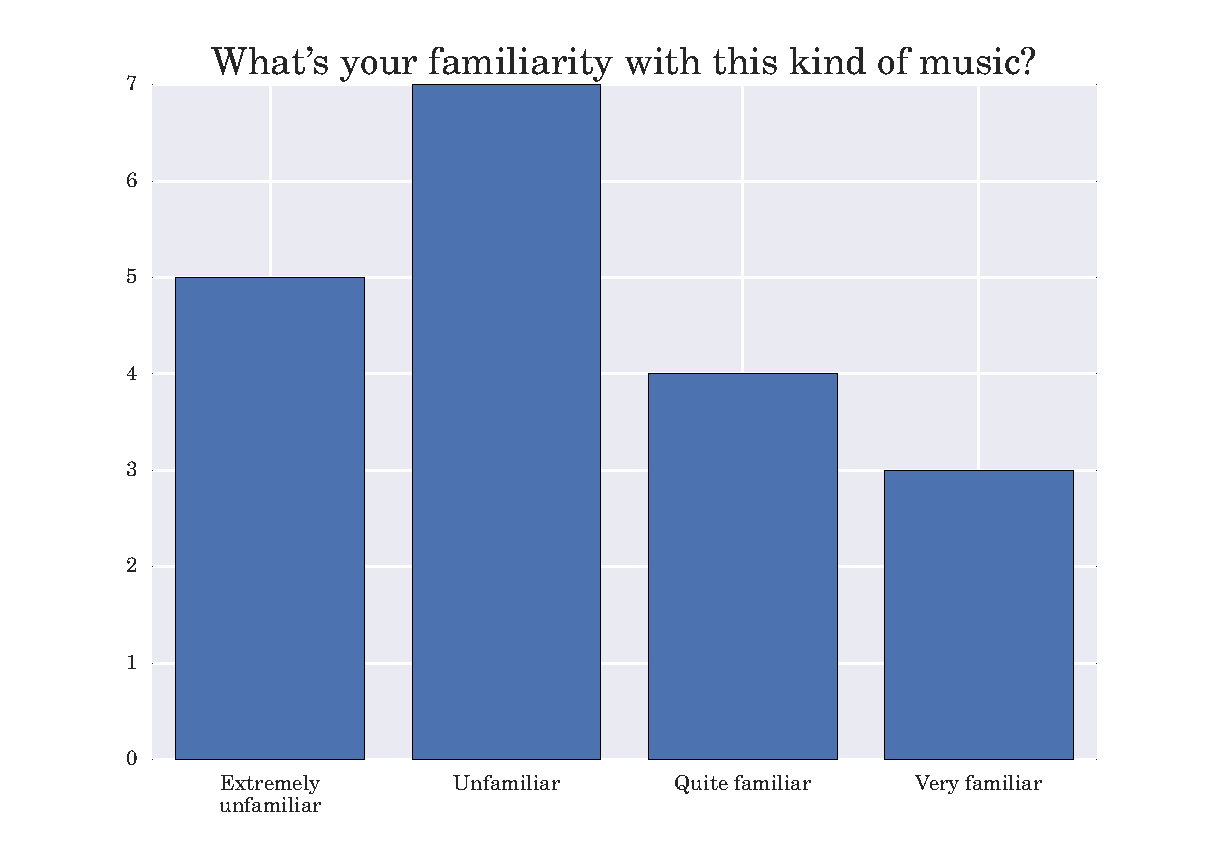
\includegraphics[scale=0.6]{Figures/musicfamiliarity.pdf}
  \caption[Evaluation results: familiarity to the electroacoustic genre of music]{Evaluation results: familiarity to the electroacoustic genre of music.}
\end{center}
\end{figure}
\\

Regarding its effective usefulness, the system was generally evaluated as useful for exploring a collection of music: \\
\begin{figure}[h]
\vspace{-0.8cm}
\begin{center}
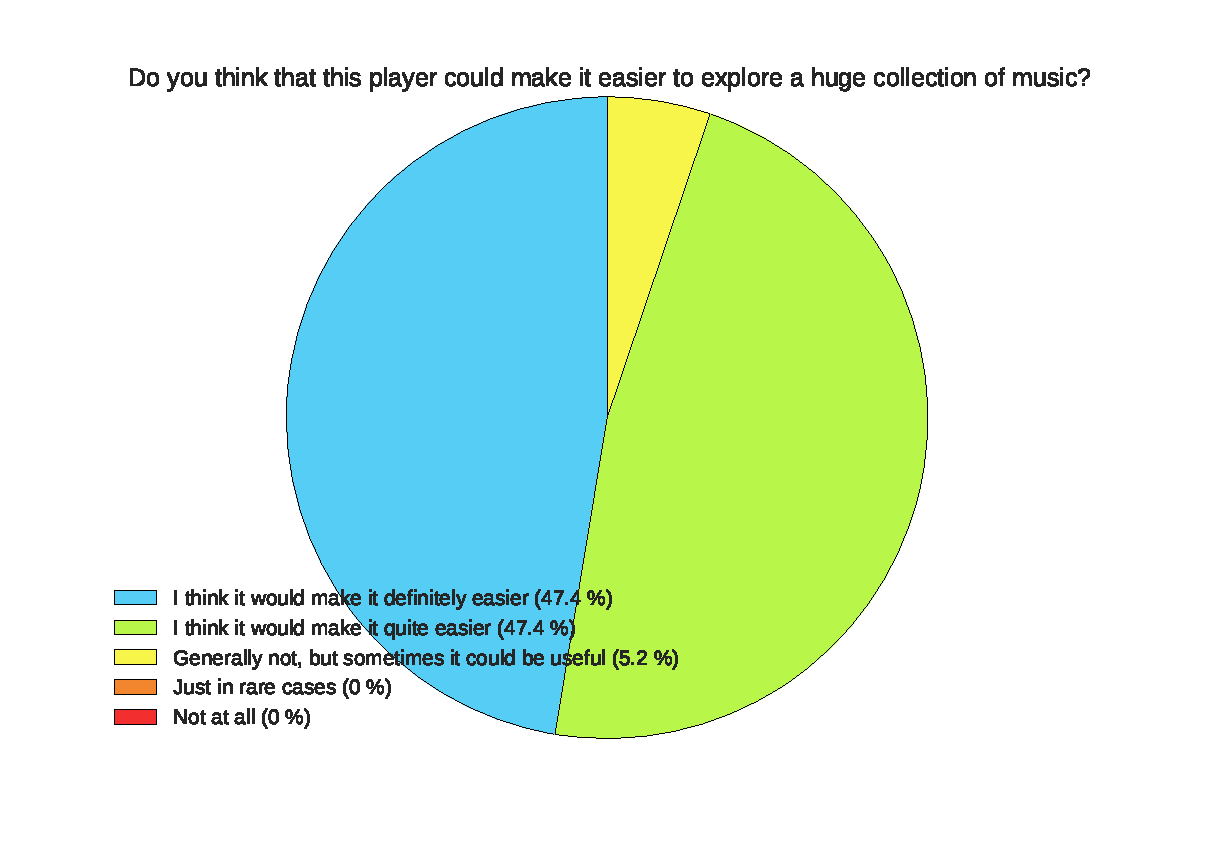
\includegraphics[scale=0.68]{Figures/usage.pdf}
  \caption[Evaluation results: usefulness of the software for exploring a collection of music]{Evaluation results: usefulness of the software for exploring a collection of music.}
\end{center}
\end{figure}
\\

while not necessarily constituting a new alternative to a traditional full-track player: \\
\begin{figure}[h]
\begin{center}
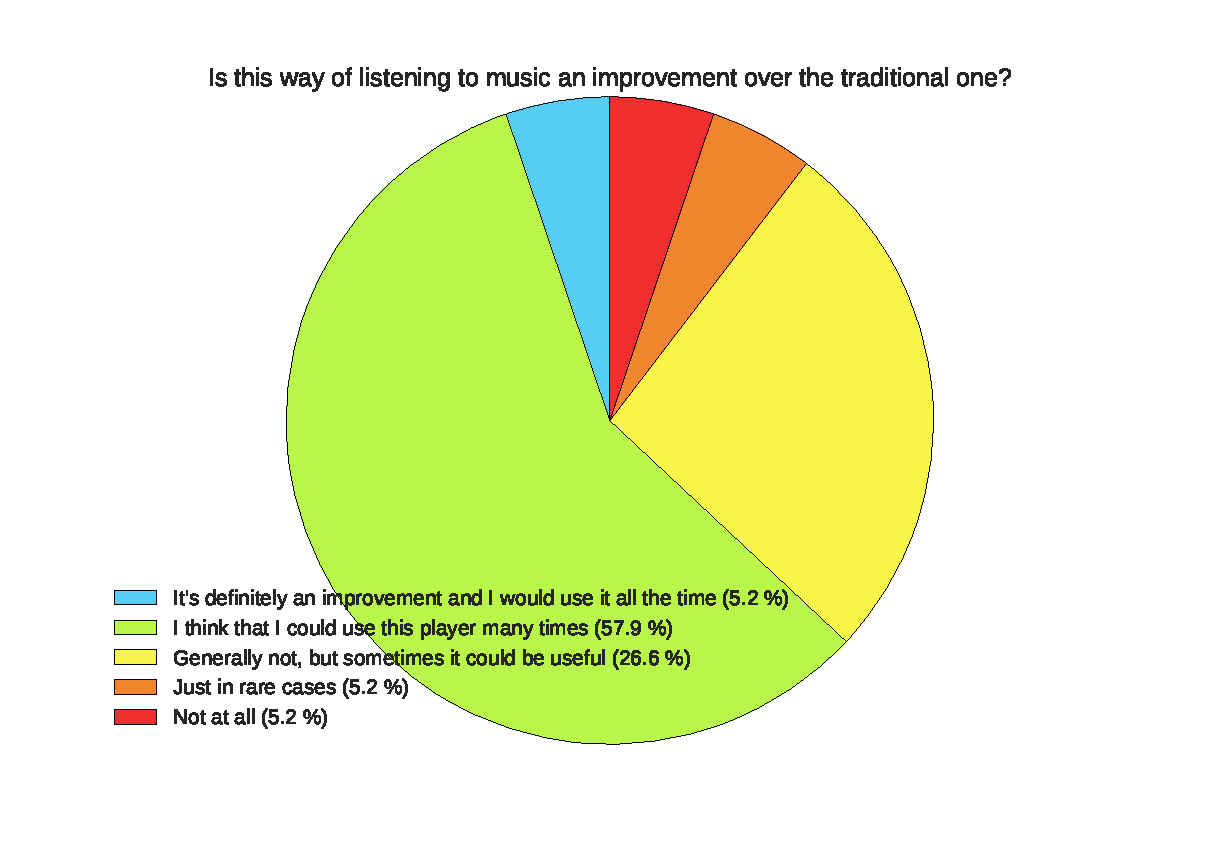
\includegraphics[scale=0.7]{Figures/improvement.pdf}
  \caption[Evaluation results: comparison of enjoyability in regards to a standard full-track player]{Evaluation results: comparison of enjoyability in regards to a standard full-track player.}
\end{center}
\end{figure}
\\

Overall, evaluation results can be considered very satisfactory: the application has succeeded both its purposes of generating an enjoyable flow of music and yet to preserve ease of use. Subjects further commented that, although generally not fully understanding the meaning of all the sliders, they were surprised to see how much the flow of music changed at the interaction with sliders. Moreover, it is interesting to observe that, despite the subjects are generally very used to music technology software, most of them were totally unfamiliar with the software developed. This may be considered as a proof that the software developed actually succeeds in its purpose of providing a new way to approach music playlist generation.

\section{Usage at exhibition} 
\begin{figure}[htbp]
\begin{center}
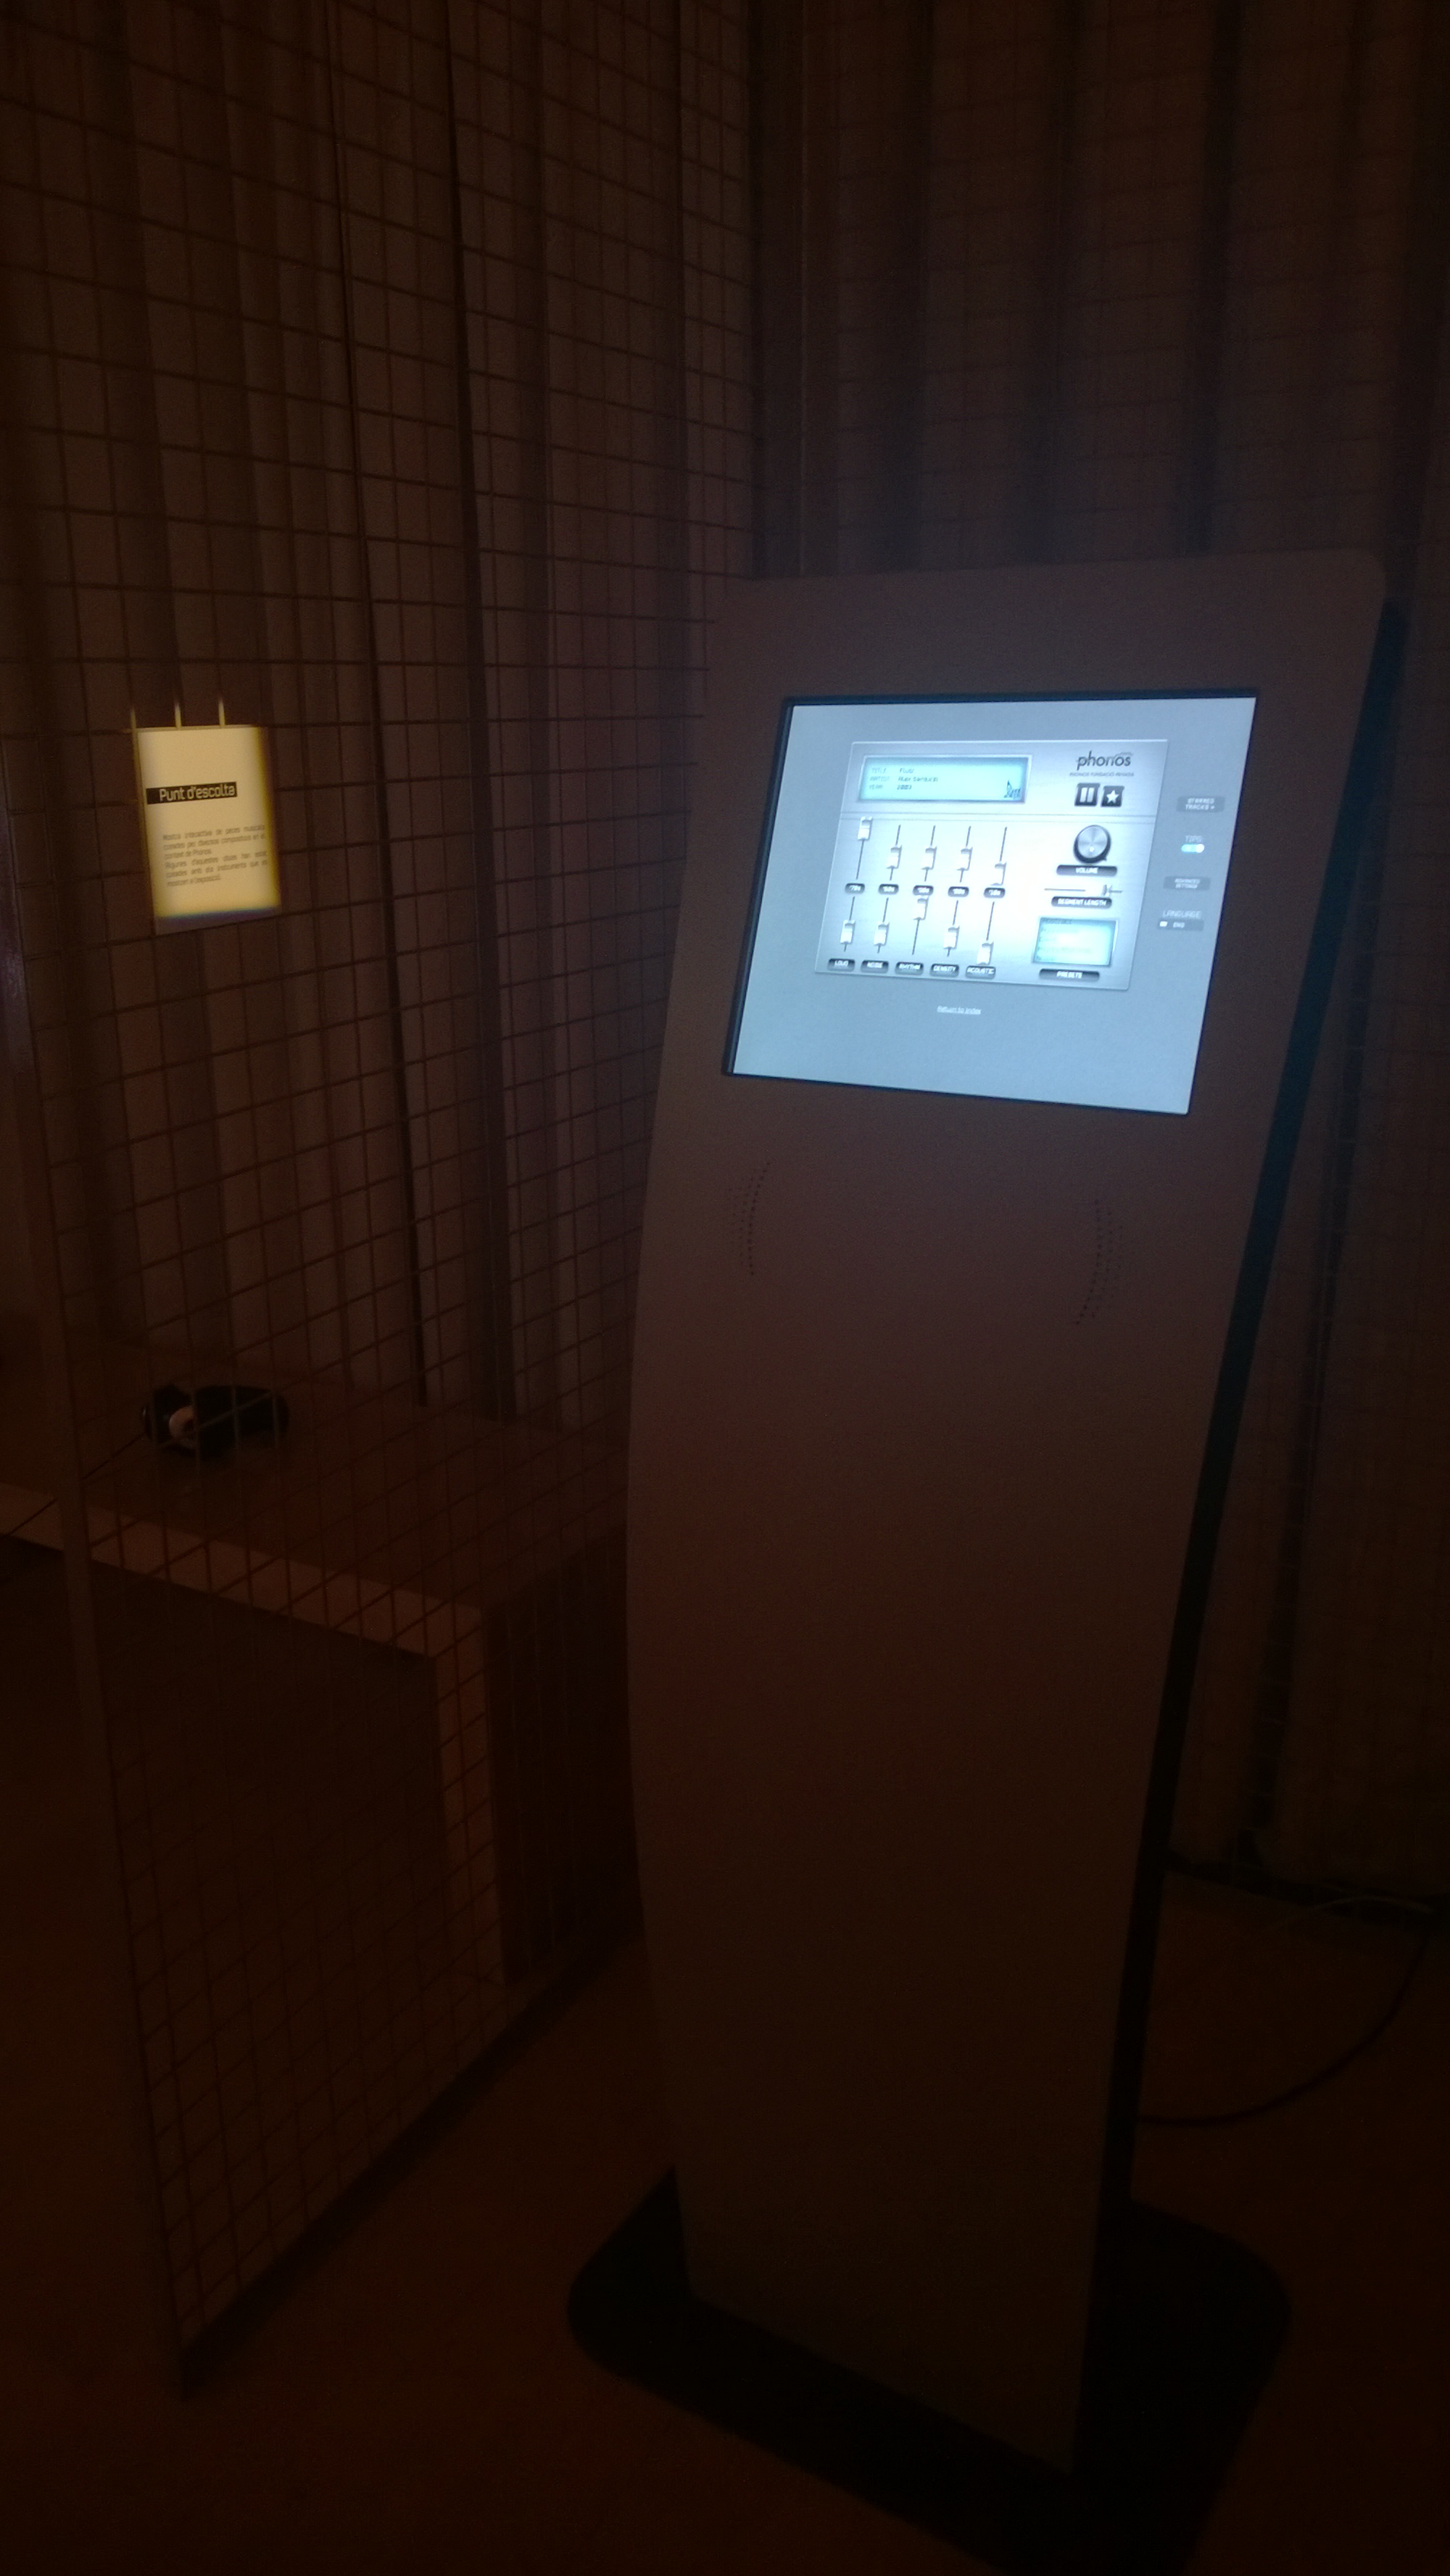
\includegraphics[scale=0.1]{Figures/kiosk1.jpg}

\vspace{1cm}

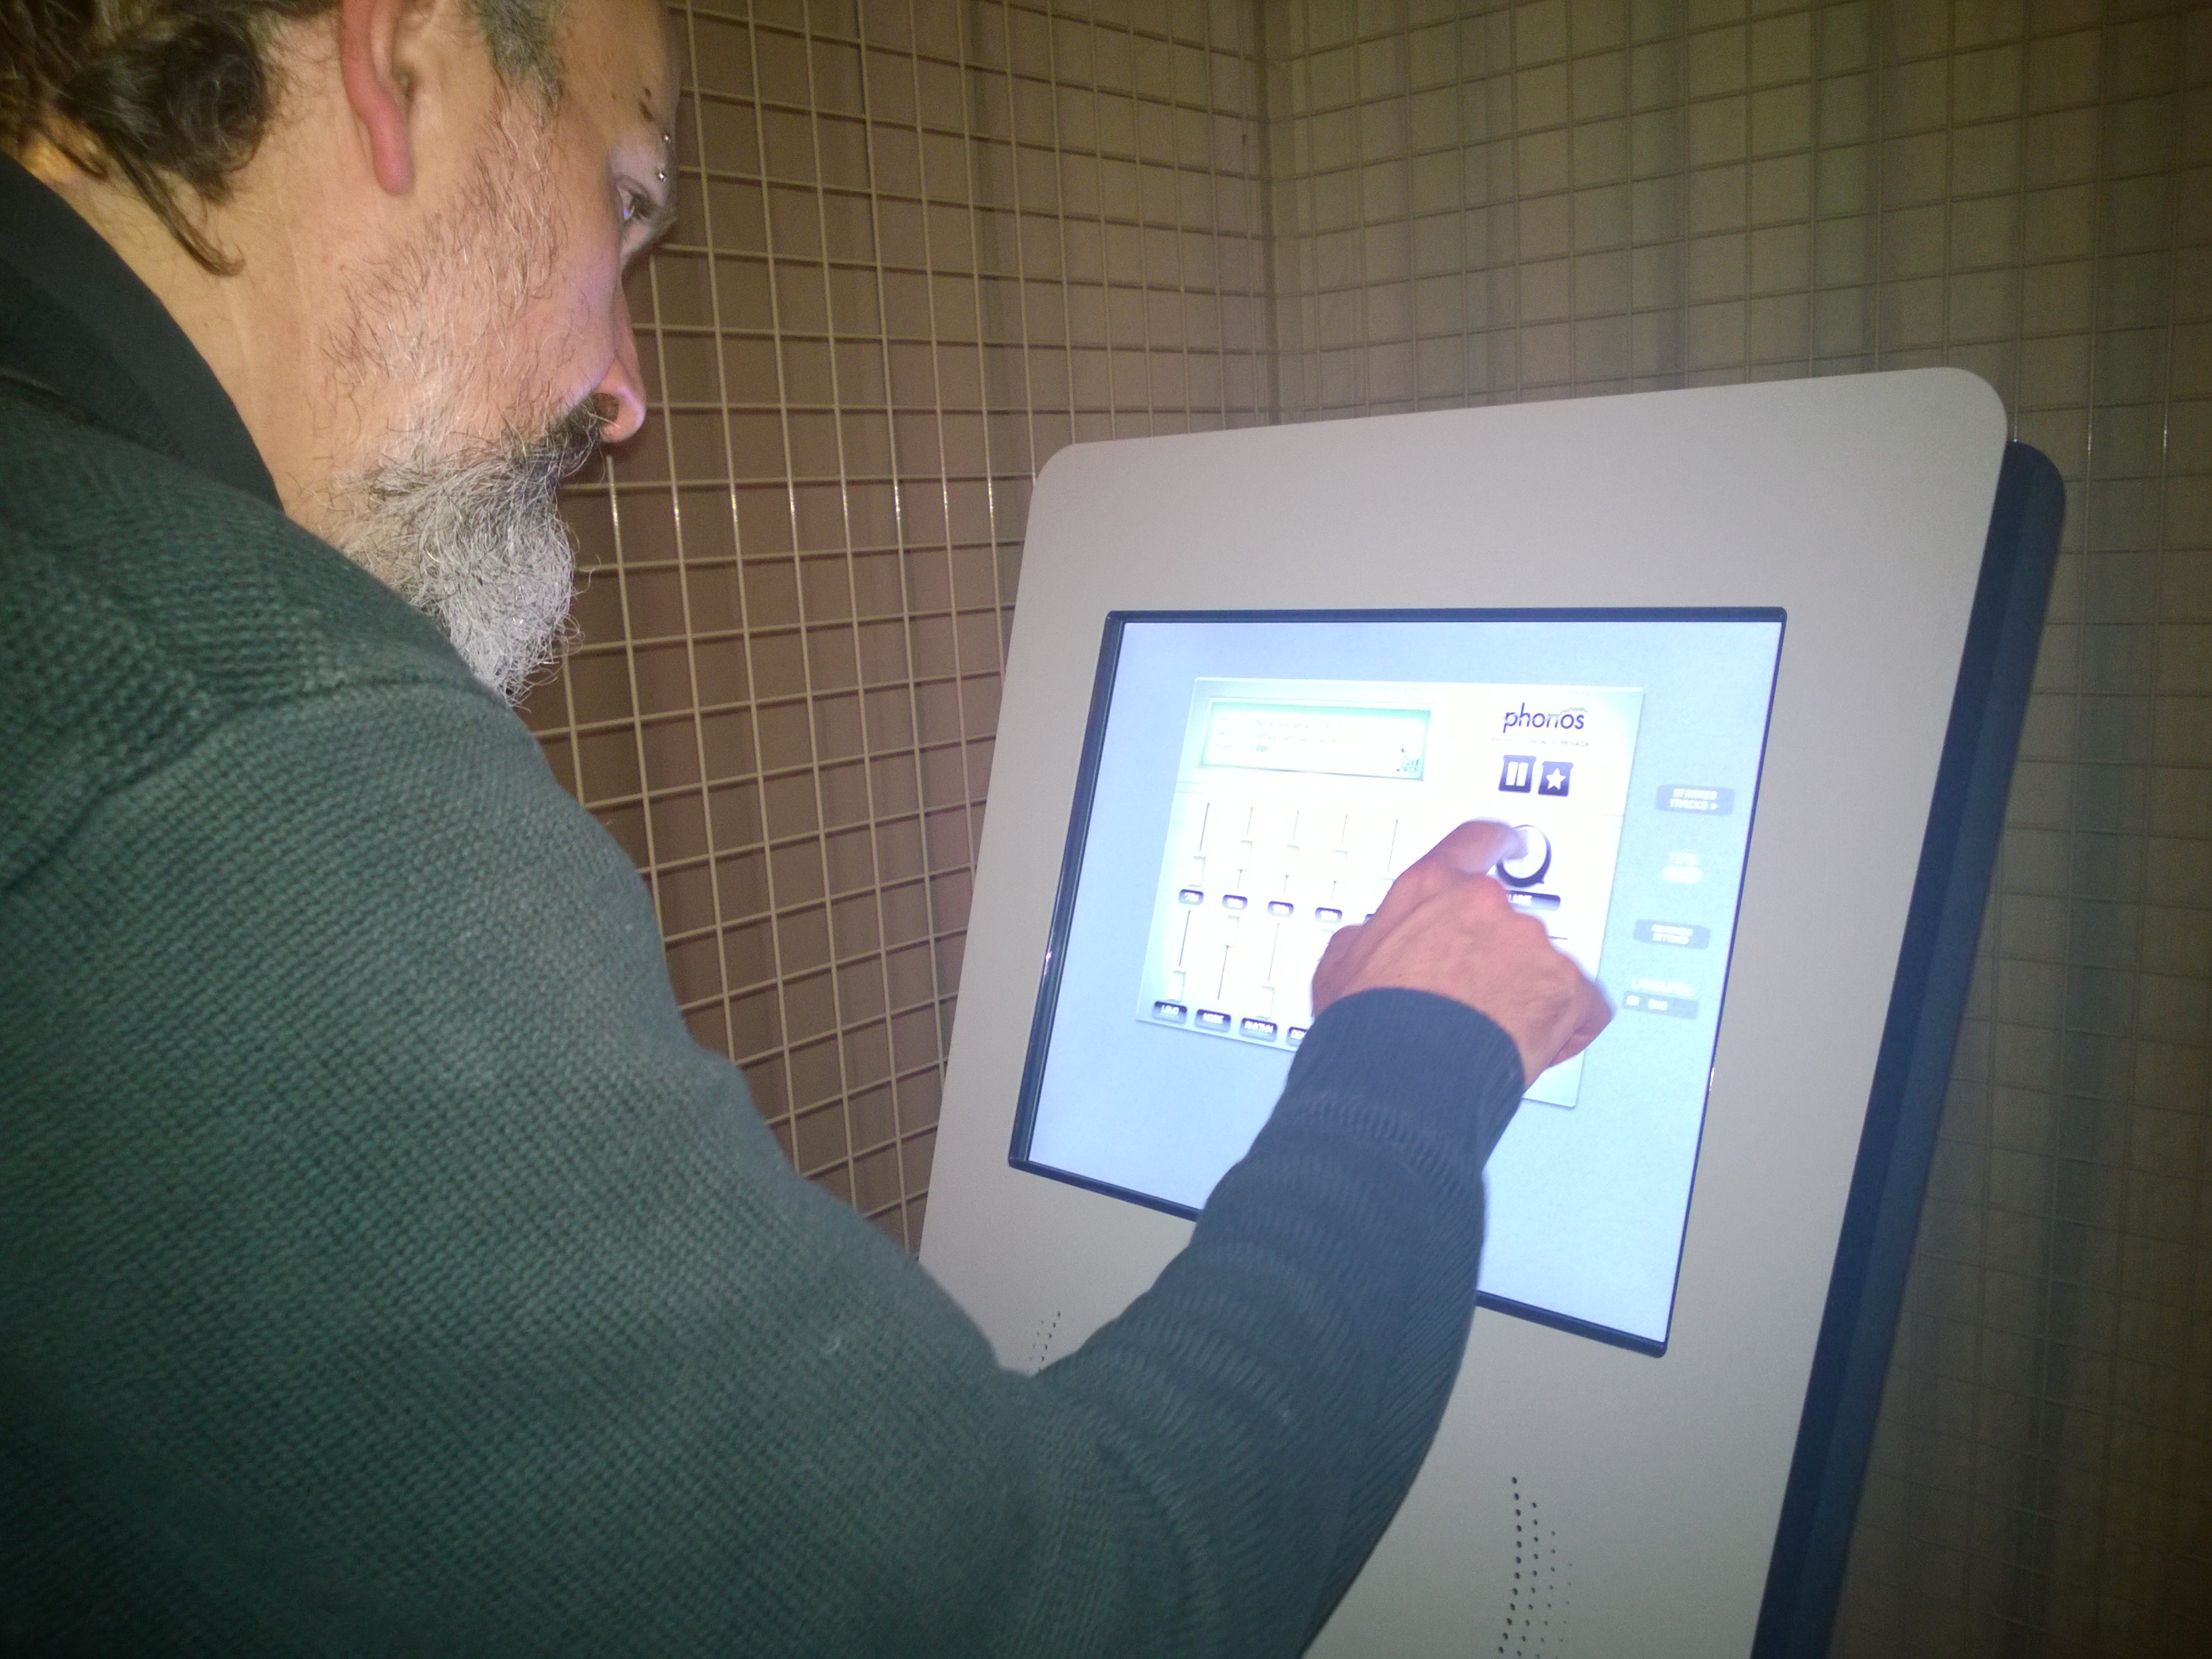
\includegraphics[scale=0.1]{Figures/kiosk2.jpg}
    \rule{20em}{0.5pt}
  \caption[Interactive kiosk at the exhibition]{Use of the interactive kiosk at the exhibition.}
  \label{fig:kiosk}
\end{center}
\end{figure}
The inauguration of the exhibition has been on December 18th 2014, at Museu de la Musica, Barcelona. Many people have interacted with the system in order to explore the Phonos catalogue of music. The system hasn't incurred in any problem. At the time of the writing (February 2015), it's still daily used by several visitors at the Museum. The interactive kiosk will be dismissed at the end of the exhibition, on late September 2015.\\
